

\section{Introduction}

In the previous chapters, we have discussed visualisation and its role in bridging the gap between data and understanding. We have applied centrality metrics to a chemical network to tell us what species are of importance and experimented in getting machine learning models to learn the chemical structure of the species in a mechanism. This final research chapter provides a brief overview of current mechanism reduction techniques, whilst providing two novel alternatives to aid the process.

Science often deals with the problem of understanding complexity. This may be accomplished through organisation and partitioning, for example, the learning of a new skill through chunking, or the parallelisation of a large mathematical problem. In cases where such methods fail, we are forced to `disregard' complexity. It is common to approximate an atom as a sphere or the value $\pi$ as 3 with little consequence to the overall result of a calculation. The process of lumping has long been used to replace a complex, changing process (e.g Quantum Mechanics or Boundary Layer Fluid Dynamics) with a simpler constant process, \citep{approx}. In such cases, an approximate analysis may be far more useful than a lengthy exact solution, or none at all. 

Similar problems of complexity can also be seen within the chemistry of the atmosphere. An example is seen within the Master Chemical Mechanism\footnote{Version 3.3.1 .} (MCM), \citep{mcm}, this contains 1228 \ch{RO2} reactions. If written explicitly all \ce{RO2-RO2} interactions would result in a total of 1507984 reactions. Instead, the MCM overcomes this problem by creating a \ch{ro2} pool, with which all \ch{RO2} species react. This results in a mechanism which preserves the quality of science with only 0.000814 of the total possible \ch{ro2-ro2} reactions.

However even with such simplifications, atmospheric chemical mechanisms have been increasing in size over the last 10 years, \autoref{fig:mcmgoogleREF}REFC1fig. With the ability to automate their construction, mechanisms with species numbers of the millions become possible. Although the existence of more-explicit mechanisms may improve the quality of science produced, they can cause problems for efficient computation, diagnosis and analysis. This chapter shall look at two methods in which we may simplify a mechanism by grouping similar species together. These are through the use of species lifetime (\autoref{sec:lifetime}) and graph-based clustering (\autoref{sec:graphreduction}).




\section{Mechanism Reduction}

As discussed, the first step to simplifying a complex task involves the partitioning data into categories. For a mechanism, we begin by looking at the reaction or species which are related to the area that is being researched. Items are partitioned into important, needed and redundant categories (described below). 

\begin{itemize}
    \item \textbf{Important} - reactions or species directly related to the topic / outcome we are interested in
    \item \textbf{Needed} - reactions/species required by the important species, such that they may perform their desired function
    \item \textbf{Redundant} - those we may remove with little or no consequence to the final outcome of the model. 
\end{itemize}



\subsection{Reaction Removal}
Since atmospheric chemical mechanism forms a numerically stiff system, a reduction in the number of reactions within a mechanism leads to a reduction in the computational burden experienced by a model each iteration forwards in time. Classically the identification of important reactions may be accomplished through the use or rate of production and loss analysis (SEC REF). This allows us to filter reactions contributing less than 5\% to the formation of any species we are interested in. Other methods using principal component analysis of the sensitivity of species (PCAS) also exist and are discussed in \cite{PCAS}.


\subsection{Species removal}
Similar to reaction removal, the removal of species is useful because the removing or combining of species inherently reduces or simplifies the reactions within a mechanism.  This method also has added benefit of reducing the size of the jacobian matrix used to propagate the chemical system forwards. For large systems which do not use a sparse framework, storing a $n^2$ matrix in memory can prove difficult.

Many methods of species reduction are possible. The simplest of these is through the use of trial and error\footnote{A tried and tested method for scientific discovery.} \citep{tur1990} (Method 1). Here the consuming reactions for a species are removed, and if the resulting deviation in results between the full and reduced mechanism is small, their results are kept. The main downside to this is that it only works on a per-species level, which may be very resource-consuming for large mechanisms.

With the use of sensitivity analysis, it is possible to remove species whose reaction are much slower than the rate-determining steps of a mechanism, \citep{frenk}. However, even after removing all slow-reacting species, those on a fast timescale remain. Here the use of Quasi-Steady-State Approximation (QSSA), \citep{QSSA}, can be used to identify species associated with fast timescale reactions. QSSA works on the assumption that such species have little to no change in concentration over time - i.e. the net flux ($\dot{v_i}$) is zero. Such an assumption causes an error $\Delta c_i$ of :
\begin{equation}
    \Delta c_i = \frac{\dot{v_i}}{J_{ii}}
\end{equation}  
where $J_{ii}$ is the diagonal of the Jacobian matrix. Here if the error for a species is small, the species may be removed from the mechanism. 


Finally, investigation of the system Jacobian can be used to identify redundant species, which is a `capable' and `efficient' method for removing most redundant reactions and species from the MCM, \citep{QSSA}. Use of a log-normalised Jacobian to determine which species can be removed is found in the connectivity method \cite{connectivity,cm}. 
Here the influence a 1\%  change in a species concentration has on the concentration of `important' species can be determined by

\begin{equation}
B_i  = \sum_j(({y_i}/{f_i})({\partial f_i}/{\partial y_i}))^2 \label{connectivity}
\end{equation}

 where $({y_i}/{f_i})({\partial f_i}/{\partial y_i})$ is element $i$ of the normalised Jacobian. Through an iterative process species with a low contribution to our important species can be found and removed.


\subsection{Lumping}

Rather than removing species or reactions from a mechanism we may combine them to form a new composite species. This is species lumping. To do this we must first consider how we determine species that are to be joined together, and then how their grouped reactions will contribute to every other species it reacts with. Some of the more general types of lumping styles are outlined below. 


\subsubsection{Chemical Lumping}\label{sec:chemlump}
Mechanisms follow protocols in their generation. This produces reaction styles that many like-structured species follow in their degradation. In determining such classes we may be able to generalise like-species reactions and group them as one.
An example of this is the Common Representative Intermediates (CRI) Mechanism (described in \autoref{whycri}).  Here the ozone production potential of the species within the MCM is used to simplify and reduce it. Species with a similar \ch{c-C} and \ch{c-H} ratio (their CRI index) are lumped into a single representative species. Alternatively, time scale analysis for species lumping has been successfully applied by  \cite{lifetime}. Here it is seen that many groups of species have coefficients that are identical or sufficiently similar, resulting based on their type. This results in a similar overall lifetime for species in the same group, allowing them to be lumped together with little overall consequence to the final result of the simulation. 


\section{Data Setup}
Unlike manual reduction, this chapter does not concern itself with the intricacies of the chemistry behind a mechanism. Instead, we search for an automated method of simplifying the mathematical structure behind a mechanism whilst preserving the quality of science it represents. Although this may not directly replicate real-world scenarios, it can provide an accurate test of the robustness of a mechanism and the equations within it. I work on the assumption that the equations describing each reaction are representative of experimental results, and in simplifying these, their usefulness in modelling the real data is preserved. This section describes the experimental setup for the experiment.


\subsection{The Mechanism}
The mechanism used is the Common Representative Intermediates (CRI) Mechanism v2.2,\citep{criv2}. This is an already reduced version of the MCM, where species are grouped based on their ozone formation potential - i.e. the \ch{c-C} and \ch{c-H} ratio of bonds. 
Reductions have been made on a compound-by-compound basis and compared to the MCM using a series of 5-day box-model simulations, \citep{cri}. 

\paragraph*{Why further simplify the CRI network?}\label{sec:whycri}

CRI v2.2 is a mechanism of 422 species and 1261 reactions. Although this is significantly smaller than the full MCM, it may still prove problematic if used within a global model - for comparison the GEOS-Chem\footnote{A global 3D model of atmospheric chemistry driven by meteorology from NASA's Goddard Earth Observing System (GEOS), \citep{geos}.} standard chemistry is approximately half the size of this, \cite{geosgit}.

\subsection{The Box-Model}
The box model used shall be an adapted version of the Dynamically Simple Model of Atmospheric Chemical Complexity (DSMACC) \cite{dsmacc,dsmaccgit}. This has had several changes which allow for multiple parallel runs, easy extraction of rates, fluxes and the jacobian matrix as well as a simple Ncurses interface for loading and parsing new files. 

The DSMACC model works by using the Kinetic PreProcessor (KPP), \citep{kpp}, to generate Fortran code, which can then be used to integrate the provided mechanism. As there were some issues presented with this a pre-pre parser code was used on the mechanism before running KPP, and a post parser on some of the files to provide the desired output. 

\subsection{Model Inputs}
The aim of this experiment is not to replicate a specific case study or scenario. Instead, we extract all non-lumped species which appear in both CRI and the MCM and provide an assortment of initial condition concentrations to cover the entirety of the input space.

To select the initial conditions there exist several sampling styles \cite{sampling}. The most common style is the random or `Monte Carlo' approach, however, this does not guarantee a homogeneous distribution of points. A lattice or grid approach is also possible, but that can result in a large number of sample points to produce a complete distribution of the input space. To overcome this a Latin hypercube can be used. This is a generalisation of the Latin square  -  a square matrix containing n items, arranged in such a way that they only appear once in each row and column (akin to a sudoku puzzle) \cite{lsq}. The experimental setup uses a Latin hypercube to define the initial condition range for 148 species and 300 simulations follow the formula below:

\begin{equation}
\text{concentration}
    \begin{cases}
      min = 10^{-8} \ max=10^{-13} , & \mathbf{if} NO,NO_2,O_3\\
      min = 10^{-8} \ max=10^{-13} , & \text{otherwise}\\
    \end{cases}
\label{eqn:icslhs}
  \end{equation}
\section{Graph based reduction}\label{sec:graphreduction}
It has been shown that the graph-based representation of the atmospheric chemical network proves useful in both the visual and mathematical analysis of simulation results (\autoref{chaptervis,chaptermetric}). It, therefore, follows that the network representation of mechanism may also have its uses in the simplification, and thus reduction, of chemical complexity.  This section will outline the basic methods of modularity (cluster) detection with the graph framework, the different methods in which this may be done and eventually apply it to a case example representative of the chemistry within the London environment.




\subsection{Graph parallels. }

\textit{
EDIT\\
Although many graph-based methods exist within the reduction realm, most of these concentrate on the generation of skeletal methods through the building of a directed tree (a subcategory of graphs from source to target) - LIST of refs and sentence of all skeletal methods. Path flux analysis (Sun et al 2010)\\
Instead, we may find ourselves applying graph theory to solve other reduction methods. For instance, we can trace back influence through connecting edges using Dijkstra's shortest path algorithm (CH2 ref) - analogous to the connectivity method, or a leave one out approach combined with PageRank to access the effects of removing a node.
}

Graph structure can be used to analyse changes of reactions or relationships between species - providing an alternative representation and method to access such data. Additionally, clustering techniques may be used to locate groups of highly connected, fast reacting/strongly related species. This has applications in both understanding the data, but more importantly chemical lumping. In creating a graph from a model simulation, we not only encode information about the chemical structure, but also the influence between species in the mechanism. By grouping species which have a strong dependence upon each other, we can simplify the provided network or mechanism. 

 \subsection{Types of Graph Clustering}
Unlike vector clustering algorithms (such as DBSCAN, UMAP and K-means - see \autoref{veccluster}), graph clustering metrics do not rely on the spatial orientation of the data to determine groups or `clusters'. Instead, these may partition the network into segments, group nodes by structural equivalence or explore the `flow' dynamics of the network.

Algorithms such as Label Propagation \citep{labelprop} and spin-glass \citep{spinglass} work by randomly assigning nodes with property or label. This property is then transferred to its neighbours. Other algorithms such as the nested block model can decompose a graph into clusters of like properties, \citep{communitygraph}. These are often grouped in the form of topological equivalence which can be either:
\begin{itemize}
    \item[-]\textit{structual equivalence} - vertices are similar if they have like neighbours, \citep{strueq}.
    \item[-]\textit{regular eqivalence} - retrieves nodes with similar connection patterns (e.g. parent - child node hierarchicl structures), \citep{regequiv}.
\end{itemize}
This works in a similar way to an autoencoder (ref auto \autoref{section}), where topological similarities are used to simplify (or encode) the network structure, in a way which it may be again decoded.

Finally, there exist a set of `flow' based models which use the network dynamics to determine the modularity of a network. These are discussed below.

\subsection{Walk/Flow-Based Clustering}
Temporal networks result in a change in the relationships between items (magnitude/type). Such changes in the network dynamics are encoded within the edges of a graph. To account for this, the primary function of a random walk or `flow' algorithms is to capture the changes between the real-world systems represented by the network.

In (SECTION SILHO) the silhouette coefficient was used to compares the vector position of clusters with regards to the distance of data points between them. Translating this to the graph framework, topological (graph) clustering defines a cluster, or module, as a region with a greater inter-cluster degree or density\footnote{The number of links or edges between items in the same group.} compared to their intra-cluster density\footnote{The number of edges to other clusters}. This results in a system, that is sorted by group, has more links between elements of the same group than with those in other groups - such patterns can be seen within the sorted adjacency matrix in (Chapter 1 REF).

Since flow-based methods are more interested in the network dynamics, than structure, the number of links or density is replaced with the time a random `walker' spends `trapped' between a set of nodes. A real-world analogy would be to view the flow of water in a slowly filling river, \autoref{fig:hpp}. Here a walker (or water molecule) traverses the entirety of the river/graph network, occasionally getting trapped between a set of nodes. Here although the water is still moving, it ends up spending more time going back and forth between a set of nodes, than exploring the rest of the network. It is these regions of stalled progress that form network clusters.

\begin{figure}[H]
    \centering
    \adjustbox{trim=0 2cm 0 1.4cm,clip}{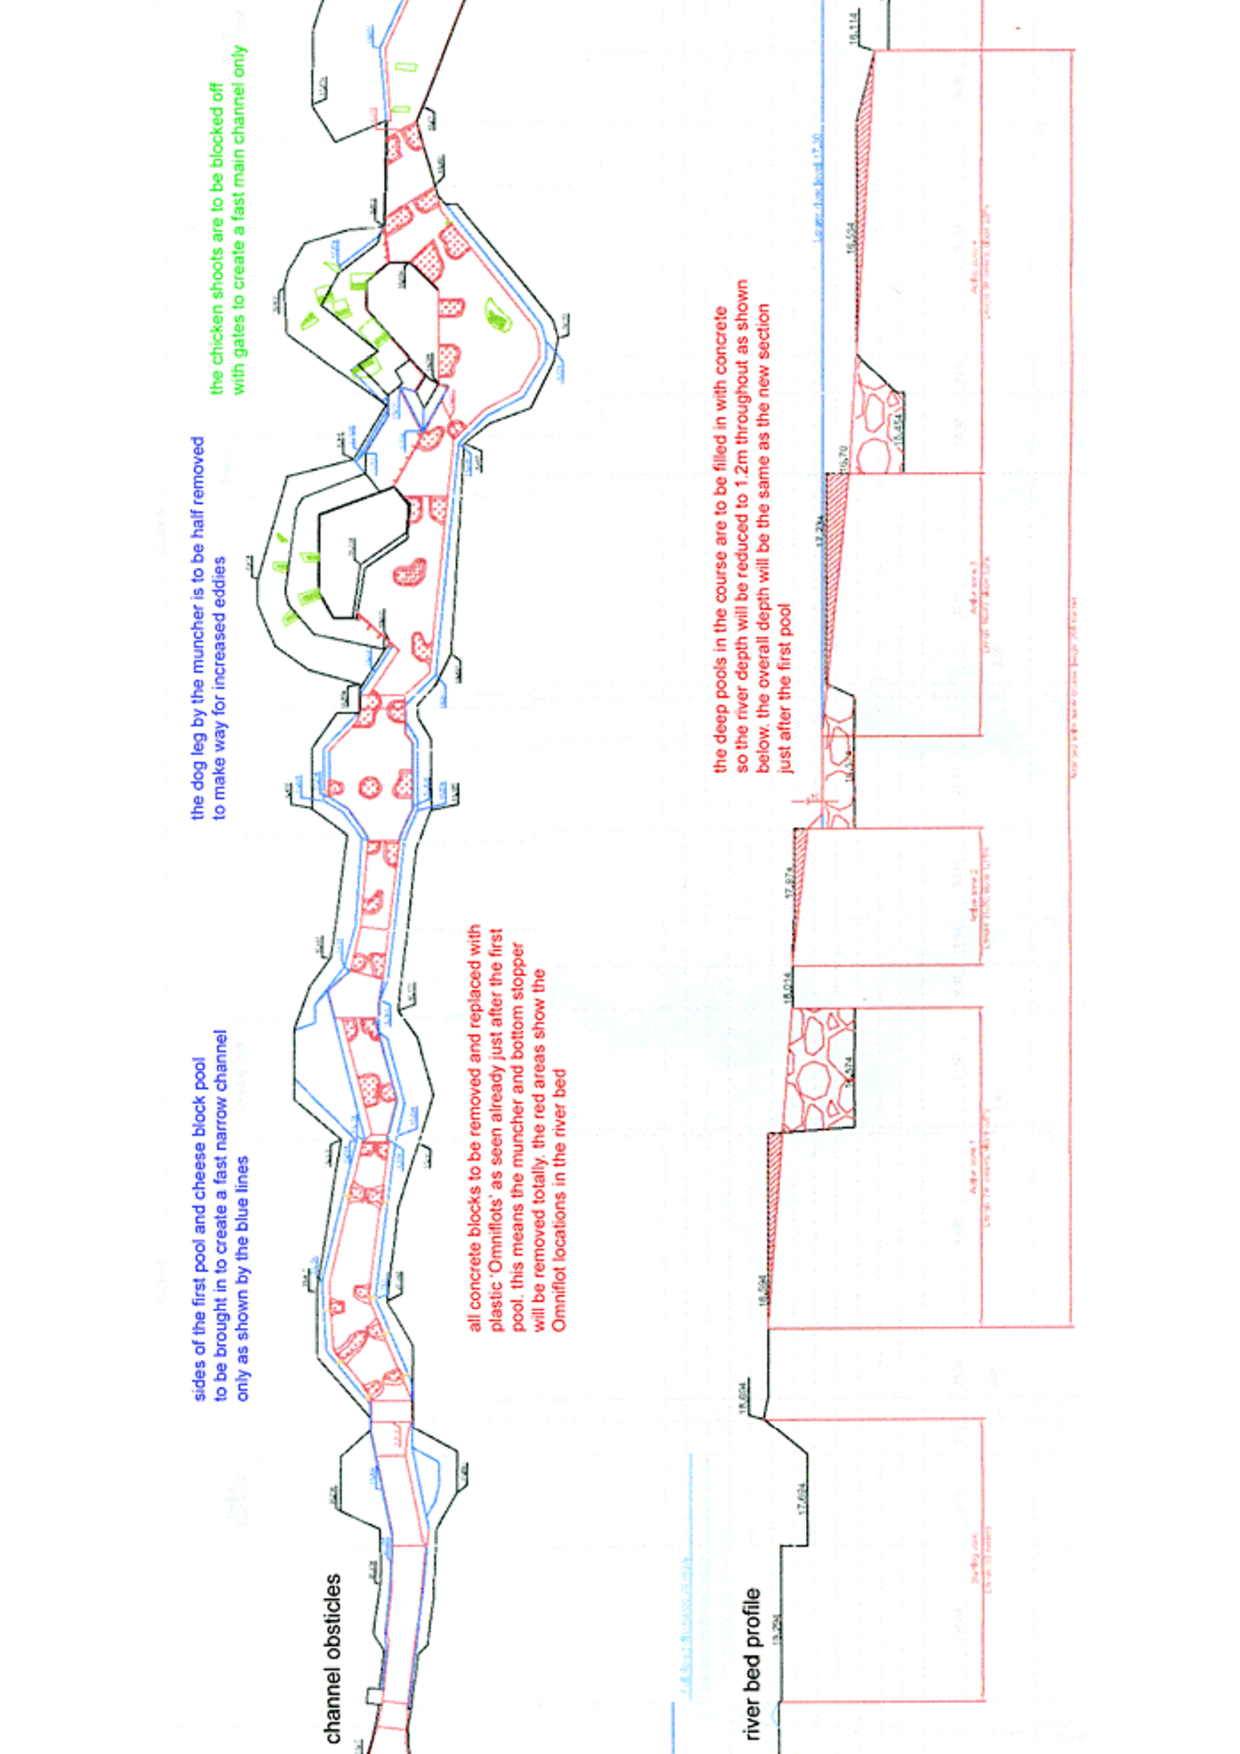
\includegraphics[height=\textwidth,angle=-90]{fig/hpp-plans.pdf}}
\caption{\textbf{The proposed plans for the change of the UK National Watersports Centre Whitewater Course (Holme Pierrepont).} Walk based clustering is analogous to the movement of a river. Clusters (or modules) are identified as areas where the `flow' becomes trapped, much like water in the pools immediately following a hydraulic jump. Source: \cite{hpp} }\label{fig:hpp}
\end{figure}

\subsection{Louvain Clustering}

The Louvain clustering algorithm is one of the most popular of the clustering algorithms due to its algorithmic and qualitative robustness, \citep{loudvain,loudrobust}. On the simplest level, this works by maximising the modularity for each configuration. Modularity is a value between positive and negative unity which measures the density of edge between inter and intra communities and compares it to an equivalent random network.
The Louvain is a hierarchical clustering algorithm, this means that after each iteration all nodes which belong to the same cluster are consolidated to form a new `grouped' item. Inter-cluster links are converted into self-links, and intra-cluster links are updated accordingly [REF INCLUDE LAYERS OF hierarchy VCRI'


\subsection{Infomap for graphical clustering }

Similar to the Louvain algorithm is the \cite{infomap}'s Infomap. Here each node within the network is assigned its module. These are then perturbed to neighbouring nodes should such a mode lead to a decrease in the map equation (a flow-based method which operates on system dynamics rather than structure - \citep{mapeqn}). The process is repeated until no further reductions are possible.

TWO LEVEL

MULITLEVERL

%Clustering algorithms seek to capture the intuitive notion that nodes should be connected to many nodes in the same community (intra-cluster density) but connected to a few nodes in other communities (inter-cluster sparsity). We compare four clustering algorithms in this study. Each scales to networks of greater than one million nodes.

% https://www.ncbi.nlm.nih.gov/pmc/articles/PMC4938516/
%
% The Infomap algorithm [18] is based on the principles of information theory. Infomap characterizes the problem of finding the optimal clustering of a graph as the problem of finding a description of minimum information of a random walk on the graph. The algorithm maximizes an objective function called the Minimum Description Length [19, 20], and in practice, an acceptable approximation to the optimal solution can be found quickly. Previous studies have found Infomap’s performance to remain stable for networks with up to 100,000 nodes [3].

% Modularity
% The modularity of a graph compares the presence of each intra-cluster edge of the graph with the probability that that edge would exist in a random graph [23, 24]. Although modularity has been shown to have a resolution limit [25], some of the most popular clustering algorithms use it as an objective function [15, 16]. Modularity is given by Eq (1),
%
% ∑k(Ekk−a2k

% Analogously, the field-of-view limit marks an upper limit on the size of communities that Louvain and Infomap can detect [36]. Infomap’s lack of a resolution limit causes it to suffer acutely from the field-of-view limit and identify smaller clusters than Louvain identifies. In this way, the resolution limit and the field-of-view limit favour Louvain over Infomap in our experiments with large communities.



\subsection{Selection Criteria for graph Clustering}

The main two criteria in selecting an algorithm for grouping atmospheric reactions are:

\begin{itemize}
    \item[1.] The algorithm can deal with a directed network - chemistry is directional.
    \item[2.] The algorithm can handle temporal data - The chemistry within a system changes depending on the time of day. This is mainly due to the change in the amount of sunlight available to photolysis reactions. 
\end{itemize}

As the InfoMap algorithm implements a directed approach coupled with a multi-level clustering approach able to capture node-layer interaction in temporal networks,\citep{infointermittent}, it makes a good candidate for the task of mechanism reduction. 

\subsection{Evaluation of InfoMap on a real simulation.}

Using the initial conditions for London from (\autoref{tab:icsmetric}), a spun up simulation run with the CRI v2.2 mechanism was run. Since this does not contain \ch{c5h11cho}, MVK, MACR or Limonene, these species are omitted from the initialisation. Following a spinup to steady-state, a graph is generated for noon after 1 day of an unconstrained run. The InfoMap algorithm is then applied to the generated graph.

The coarsest level of clustering is shown in \autoref{fig:iml1}. Here nodes are coloured by their cluster, and approximate polygon hulls surround the nodes closest to the median cluster centre. Much like the findings in (CHAPTER STRT), it is seen that different sections of the graph network represent different types of chemistry - for example, hull 4 contains aromatic species, hull 2 contains the products of linear alkanes and hull 3 contains the terpenes.


\begin{figure}[H]
  \centering
  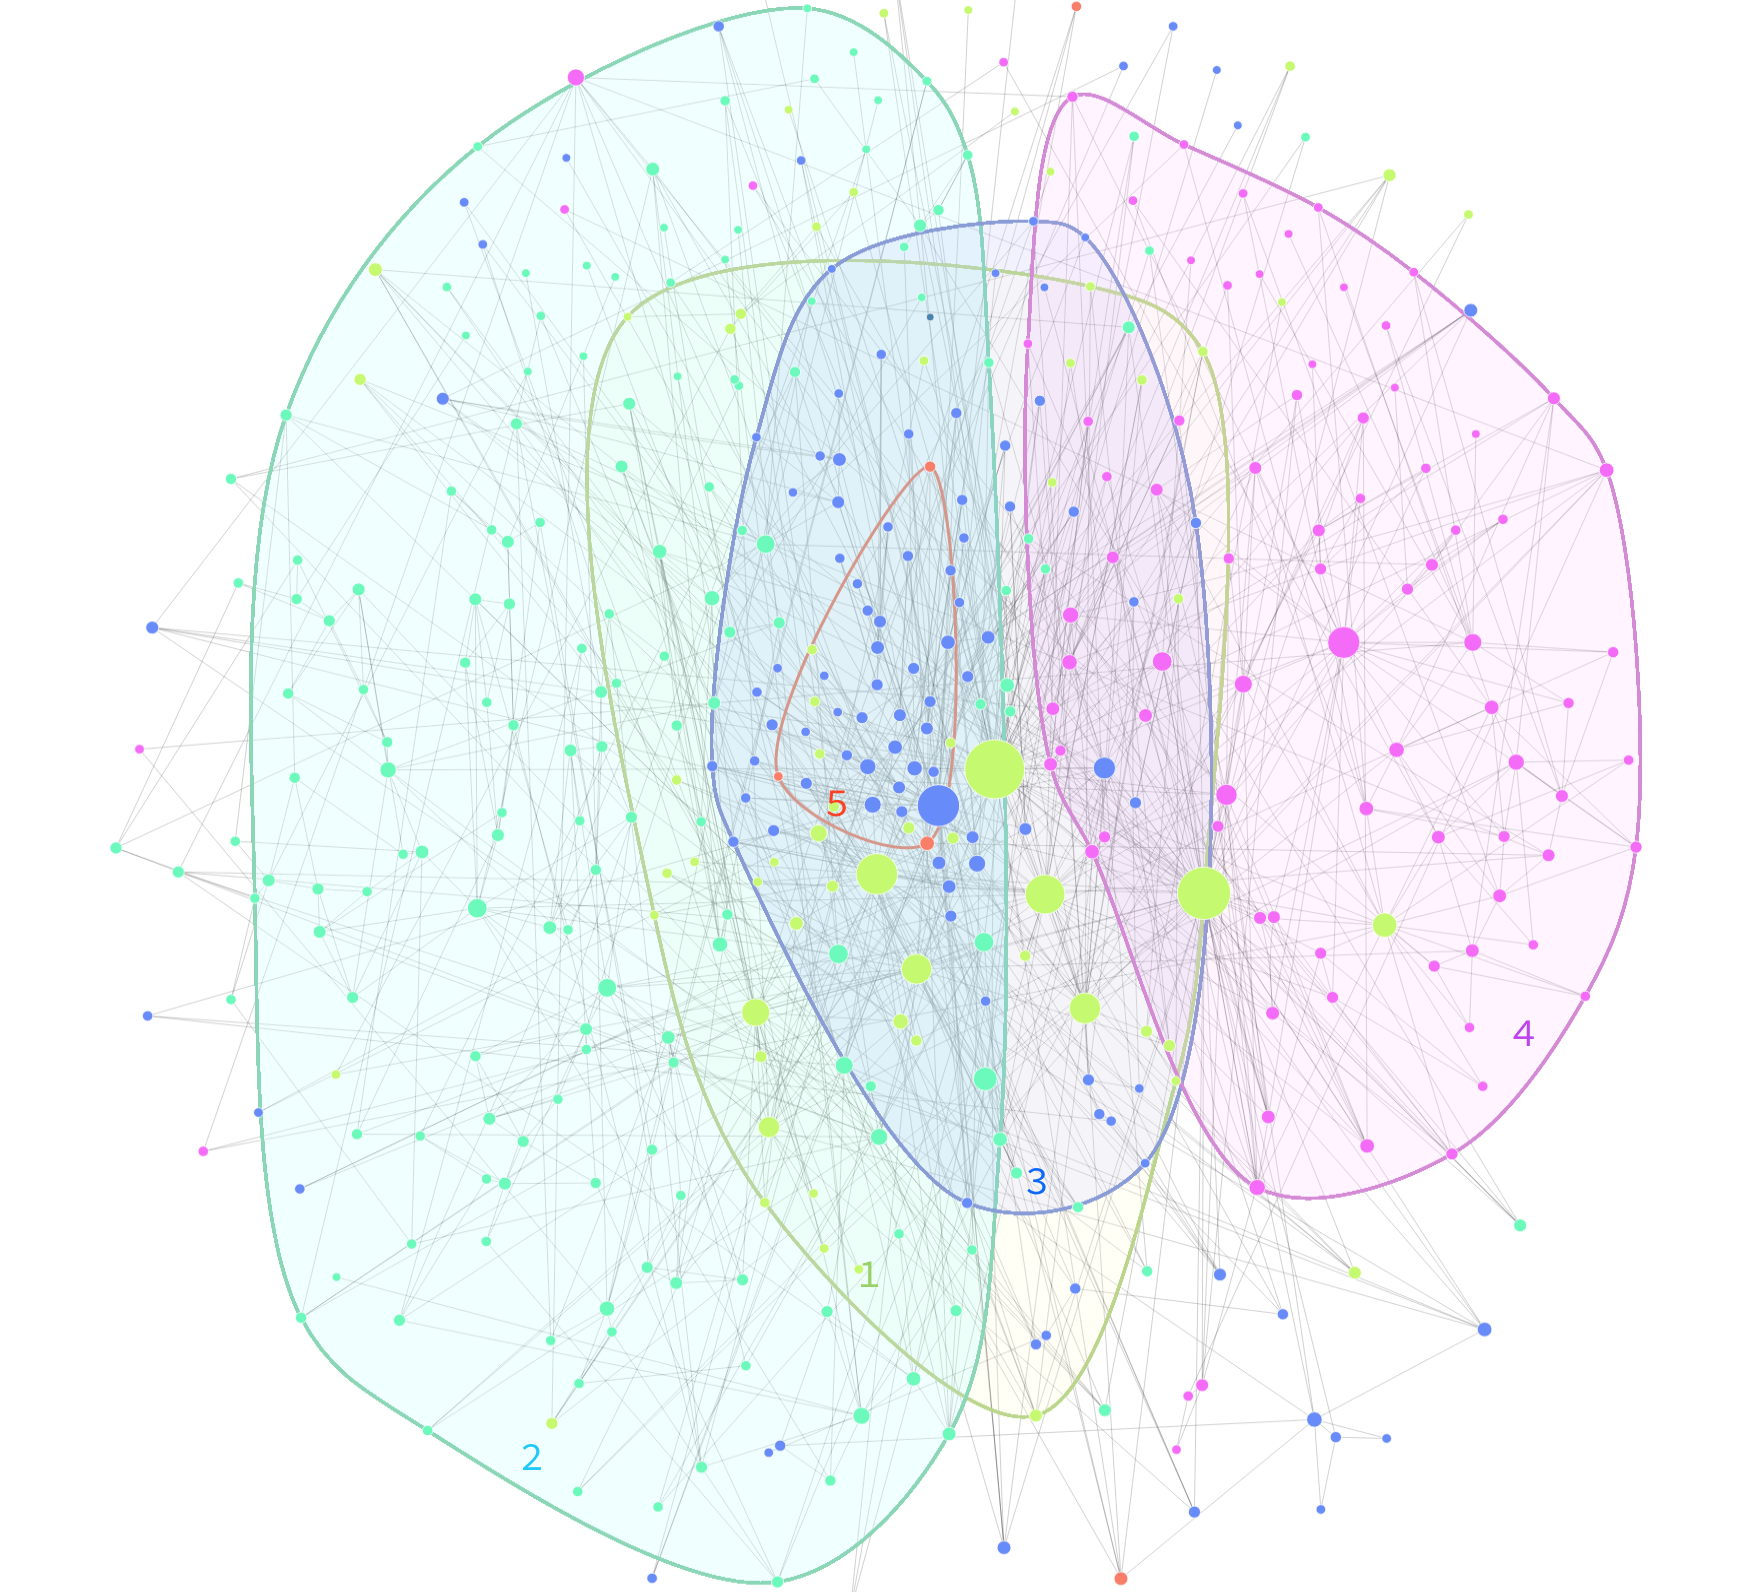
\includegraphics[width=\textwidth]{fig/crigroups.png}
  \caption{\textbf{A graph of CRI v2.2 showing the hulls of the first level of hierarchical clustering.} Nodes are coloured by the splits in branches, and the hulls enclose the nodes which lie within 95\% of the (median) centre of the cluster.}
    \label{fig:iml1}
\end{figure}

Since the InfoMap provides a finer level of clustering which has originated from this, it is important to evaluate this. Using a graph-hull approach, as in \autoref{fig:iml1}, becomes cluttered and unusable. Instead, a bubble plot may be used. Although this sacrifices the ability to view links, it allows for the complete overview of the hierarchical structure. In \autoref{fig:imbubble} shows the nested structure of each clustered group. In an electronic mail correspondence with \cite{correspondance} the origin of the naming convention of reduced species was explained. Using this, individual nodes are coloured by their prefixes. This allows the further categorisation of the species structure within each category. 

\begin{figure}[H]
  \centering
  \includegraphics[width=.95\textwidth]{fig/imapbubble.pdf}
  \caption{\textbf{Species structure within each cluster.} A nested bubble chart is used to show the full hierarchical structure of the mechanism. This allows us to evaluate the species structure/type that has been extracted in each level of the hierarchical split. Node sizes are representative of the $\log_{10}$ number of walkers that have become trapped by the flow algorithm at a location. }
    \label{fig:imbubble}
\end{figure}


 \twopagepicture{t}{t}{mechanism_lumping/tree.pdf}{\textbf{A radial treemap showing the hierarchical clustering of the CRI mechanism.} The simulation results used are representative of the chemistry within London at Noon local time and generated using DSMACC and the InfoMap algorithm.
 }{fig:imap2page}{1.0}{0}


\subsubsection{Species type and clustering}
Although the nested bubble chart is an intuitive way to represent groups within a graph, a tree approach is more suited to revealing the hierarchical structure of the network, \autoref{fig:imap2page}. Here branches are numerically labelled on each level, allowing us to navigate the structure using a sequence of numbers (e.g. to get to 1.5.\ch{c4h6} we take the first branch from the centre, followed by the fifth branch after that).

This split notation allows a general overview of the mechanism structure, as well as the reasoning/process of the clustering algorithm. The first level split in \autoref{fig:iml1} shows branches 1,2 and 5 to have origins in the linear (n-) alkane species. This can be seen through both the emitted species (bold) and the \emph{RN} prefix of the species. Here the linear alkanes can react with OH to extract hydrogen and then from a \ce{RO2}, or produce a carbonyl \emph{\ce{CARBxx}}, which can then go on to produce the \emph{\ce{RNxxO2}} peroxy radical.

Except for benzine in 2.14, branches 3 and 4 contain the aromatic species in the network.  Branches 4.\{2,5,9,11\} all consist of \emph{\ce{RAxxO2}} species, which are the product of the addition of OH to toluene/benzine ringed species. 4.\{1,7,8\} and 1.5 contain peroxy radicals formed from the degradation of conjugated dienes (two alkene groups separated by a single bond, where some sharing of electrons may occur) \emph{\ce{RUxxO2}}. For the CRI v2.2 mechanism these are only isoprene and 1,3-butadiene. Such peroxy radicals often go on to form unsaturated carbonyls, as denoted by \emph{\ce{UCARBxx}}.

Branch 3 contains the monoterpenes. This can be seen in 3.\{2,5\} ($\alpha-$pinene) and 3.6 ($\beta-$pinenen). Here peroxy radicals formed from the reaction with the e\textbf{n}docyclinc\footnote{Inside the pinene ring.} and e\textbf{x}docyclinc\footnote{Outside the pinene ring.} double bonds of $\alpha-$ and $\beta-$ pinene are denoted with the prefix \emph{\ce{RTN}} and \emph{\ce{RTX}}.

The \emph{\ce{RIxxO2}} prefix was originally used for the peroxy radicals iso (`i-') alkanes and their carbonyl products - branches 3.\{1,4\}, however, they tend to mainly be used for smaller branched precursors which produce acetone (\ch{CH3COCH3}) as a major product in their oxidation chain (branch 3.1). As acetone is a particularly unreactive carbonyl, the fact that it is water-soluble means that they may be washed out of the atmosphere by precipitation, \citep{acetonerain}. This may have been seen to interrupt the ozone formation process under regional-scale photochemical smog conditions in north-western Europe [ - from M.Jenkins PAPER? do you know what this is ].

Finally, since the CRI index is representative of the oxidation potential it is common to see species containing the CRI value within a cluster. Cluster typically contain a combination of carbonyl (\ch{R(=O)R}',\emph{CARBxx}), hydroperoxy (\ch{R-OOH},\emph{RxxOOH}), peroxy (\ch{ROO.}, \emph{\ce{RxxO2}}) and nitrate (\ch{R-ONO2},\emph{\ch{NO3}}) groups. For the lumped species, it can be common for a \ch{RO2} species to react with NO or \ch{NO3} to produce a carbonyl with a CRI index of two values lower. This can be attributed to the loss of oxygen and the formation of a double bond? (what is the long reaction for the MCM, it seems less direct). Similarly, a reaction with NO or \ch{ho2} can produce a hydroperoxy or nitrate species, which in turn react with OH to produce the an equivalent carbonyl.


%% good paper for introduction acetone
% 
% \subsubsection{Inter and Intra links}
%  Typically the quality of clustering can be assessed using the adjacency matrix of a graph. In sortting the axis by cluster groups, squares of high density inter connections should become apparent in an adjacency heatmap. Unfortunately for an atmospheric chemistry mechanism, the size and sparseness of a graph, makes this an infeisable method to visually acess the nodcluster node ratios. Instead we can adapt the nodes presented by the treemap in \autoref{fig:imap2page} and replacing the hierarchical structure, with one representing the original graph.
% 
% 
%    \begin{figure}[H]
%      \centering
%      \includegraphics[width=1.1\textwidth]{fig/treeplot.pdf}
%      \caption{\textbf{The L1 cluster graph using the tree layout from \autoref{fig:imap2page}. } This can be used to explore intra cluster relationships.  }
%          \label{fig:imtreeplot}
%    \end{figure}
% 
% 



 \subsubsection{Number of clusters}
Sometimes it may be required to have preset (target) number of clusters. The InfoMap algorithm contains a \emph{preffered number of modules} parameter which can either terminate the algorithm early, should the number be reached (or continue splitting if it has not). Since we are interested in merging smaller numbers of nodes, this can be seen as a useful parameter to have. However, in selecting a number too large, (e.g. 200 clusters, which should result in groups of 2-3 nodes), it is seen that much of the hierarchical information from the network is lost, \autoref{fig:im200}. It is for this reason that forcing the number of nodes without reason will not be attempted.


  \begin{figure}[H]
    \centering
    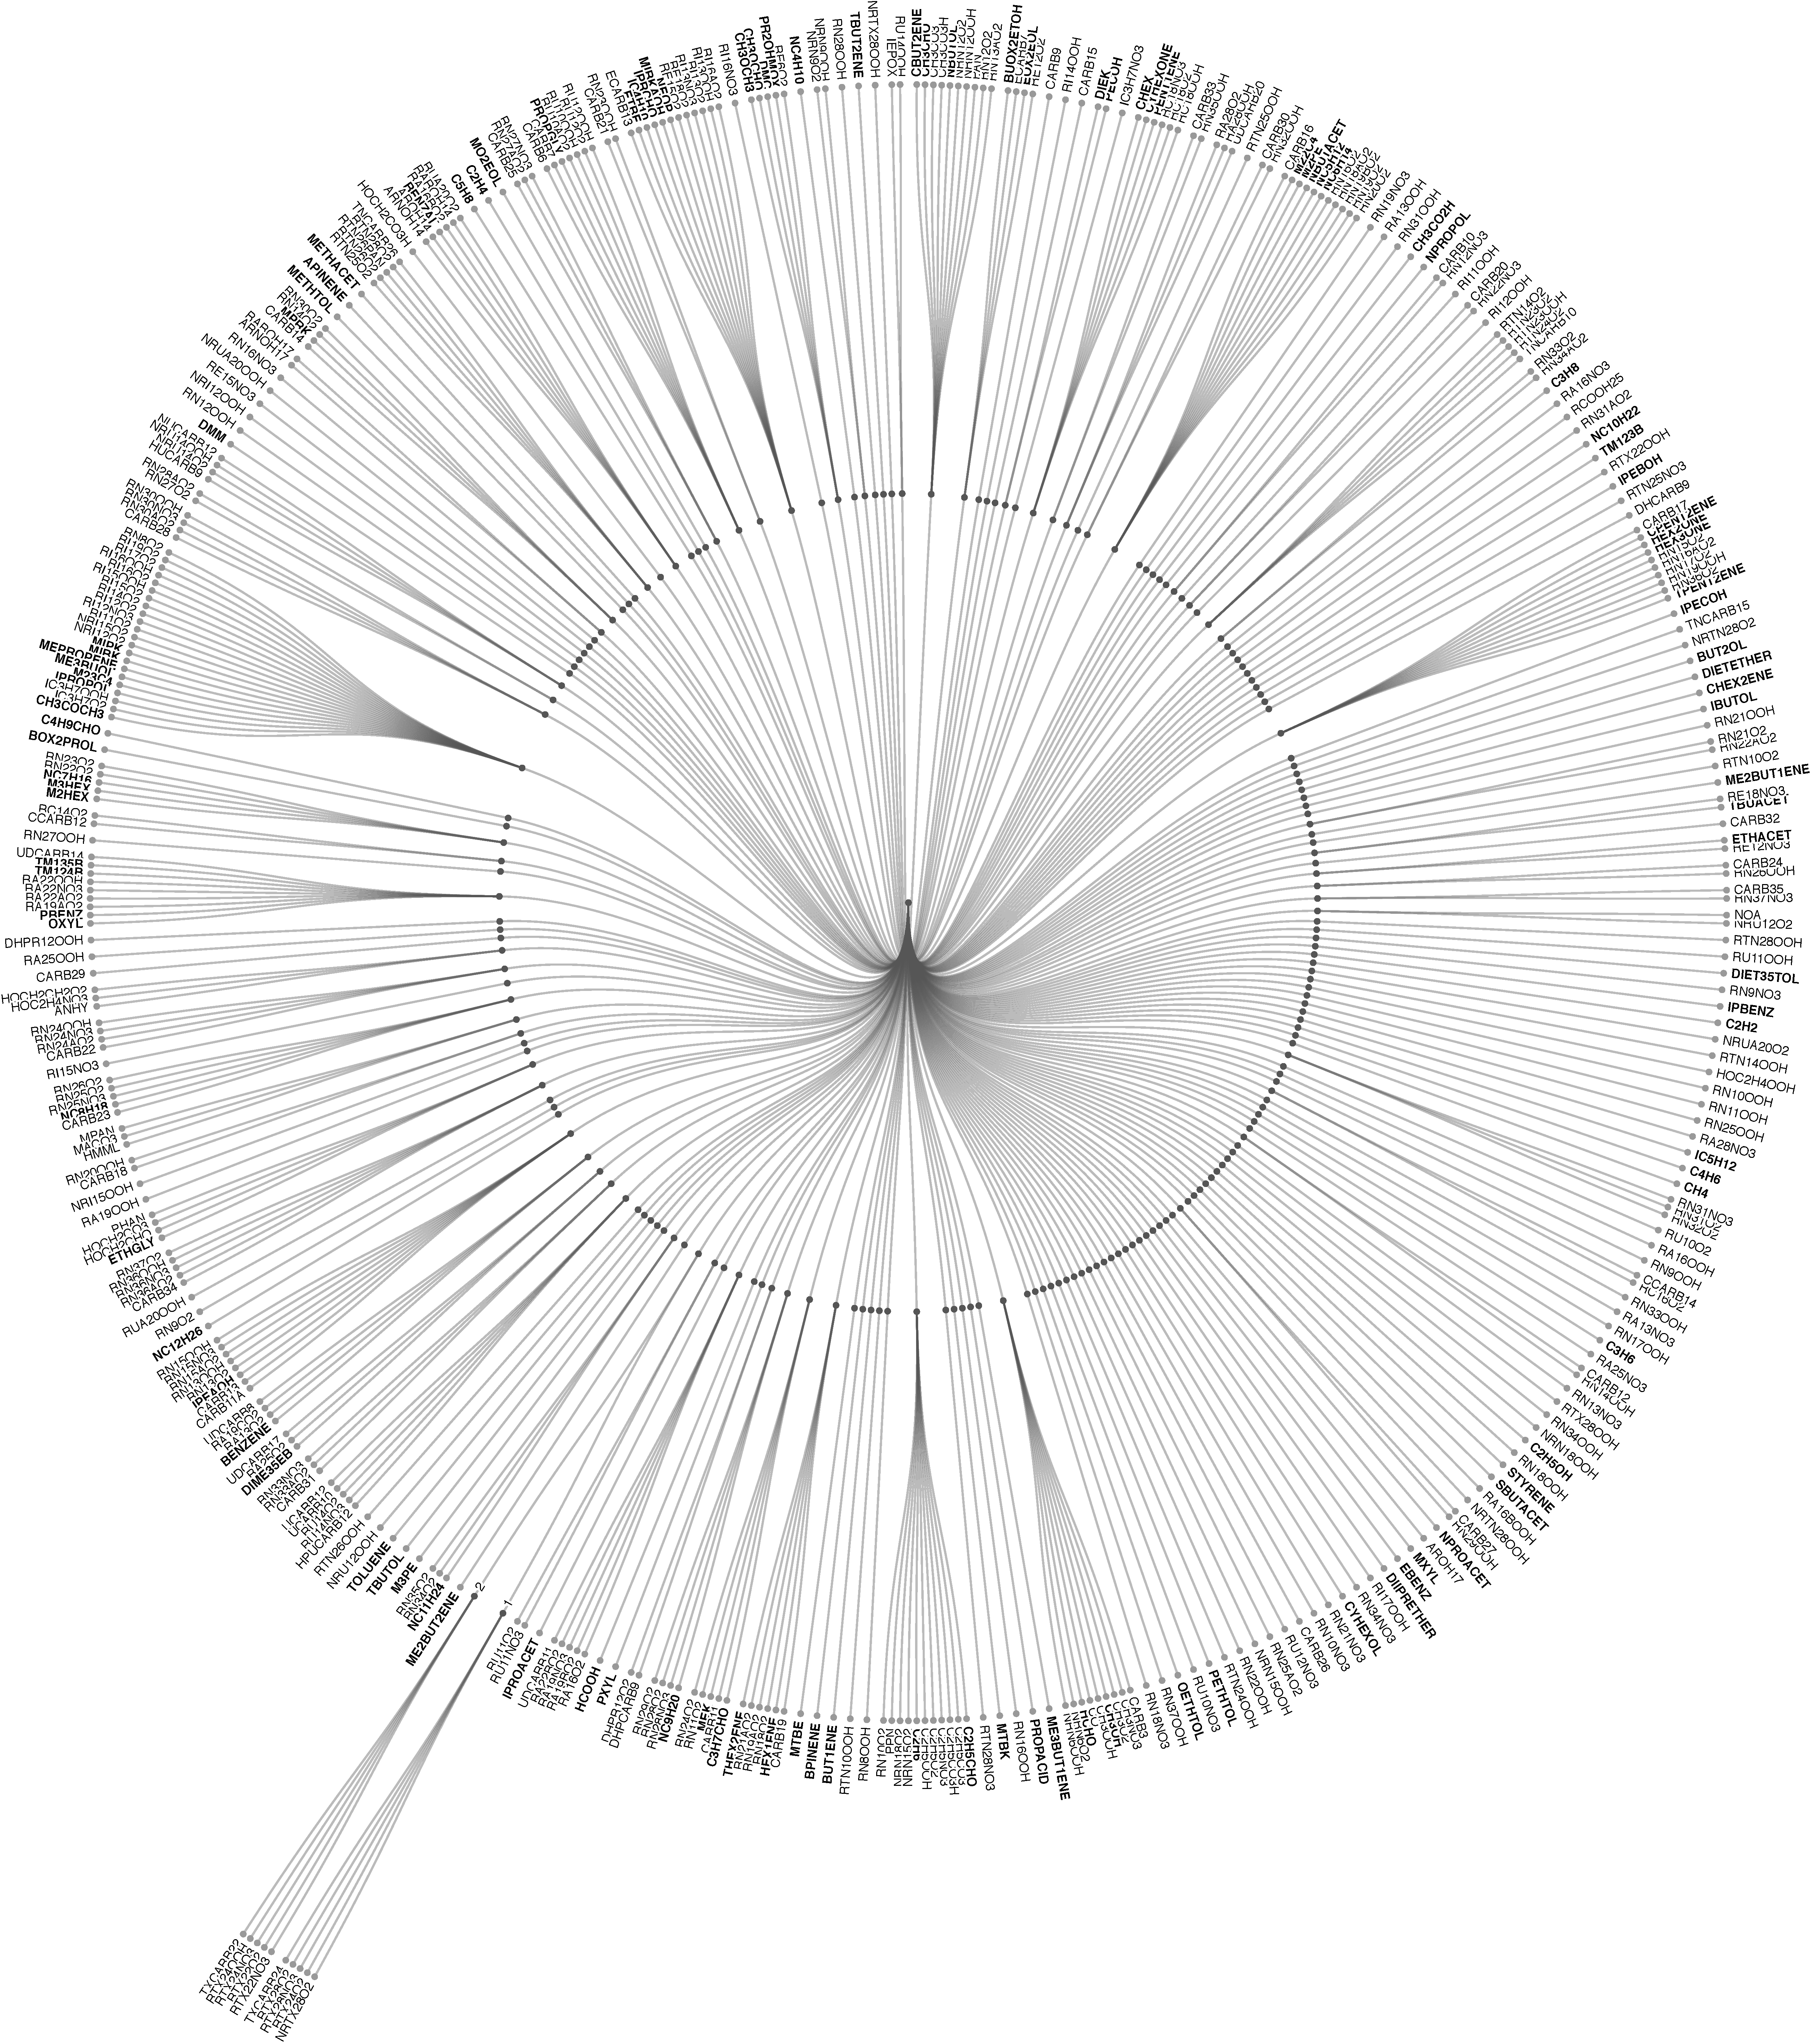
\includegraphics[width=.8\textwidth]{fig/manygroups.pdf}
    \caption{\textbf{A radial tree of the InfoMap algorithm with a forced number of groups.} Here a loss of hierarchical structure can be seen when compared to \autoref{fig:imap2page}. By setting a high number of required clusters, many species are grouped by themselves, which does not provide a useful output for mechanism lumping. }
        \label{fig:im200}
  \end{figure}




















%


\section{Results}

In order to get a representation of the mechanism we run 300 randomly initiated scenarios. The experiemental setup is one such that it is possible to add more datapoints at a later date. From each simulation the no diagonal elements of the jacobian are used to construct a graph representative of the aggregated hourly means of the simulation output. Each of these graphs is then run through the infomap algorithm and a grouping/clustering produced. To select the best possible grouping, each infomap is run 100 times, where the result with the best fit (shortest codelength) is taken - this is an optional parameter on the algorithm.

\subsection{The co-grouping network}

To aggregate the groupings produced by each algorithm an $n\times n$ matrix is created for each of the $n$ species in the mechanism. This is treated as a graph relational matrix, whereupon if species A is in the same group as species B, then a link (or value +1) is added to the [A,B] (A\ce{->}B) and [B,A] (B\ce{->}A) column. Using this matrix format it is possible to then generate a graph showing the relationship between species that were clustered in the same group.

This relational matrix can then easily be converted into the network format: \autoref{fig:infomapprune}a. Starting with this it is then possible to filter edges below a certain weight, \autoref{fig:infomapprune}b-d. Finally isolates (nodes with no links) are removed, leaving only those clusters where each species has a strong relationship between every other. 

In the context of this section we select only relationships that appear in over 45\% of all the clustered simulation runs. The reasoning behind this is that there may exist a set of pairing that only appear either during the day or night.  

\begin{figure}[H]
\begin{subfigure}[t]{.5\textwidth}
  \centering
  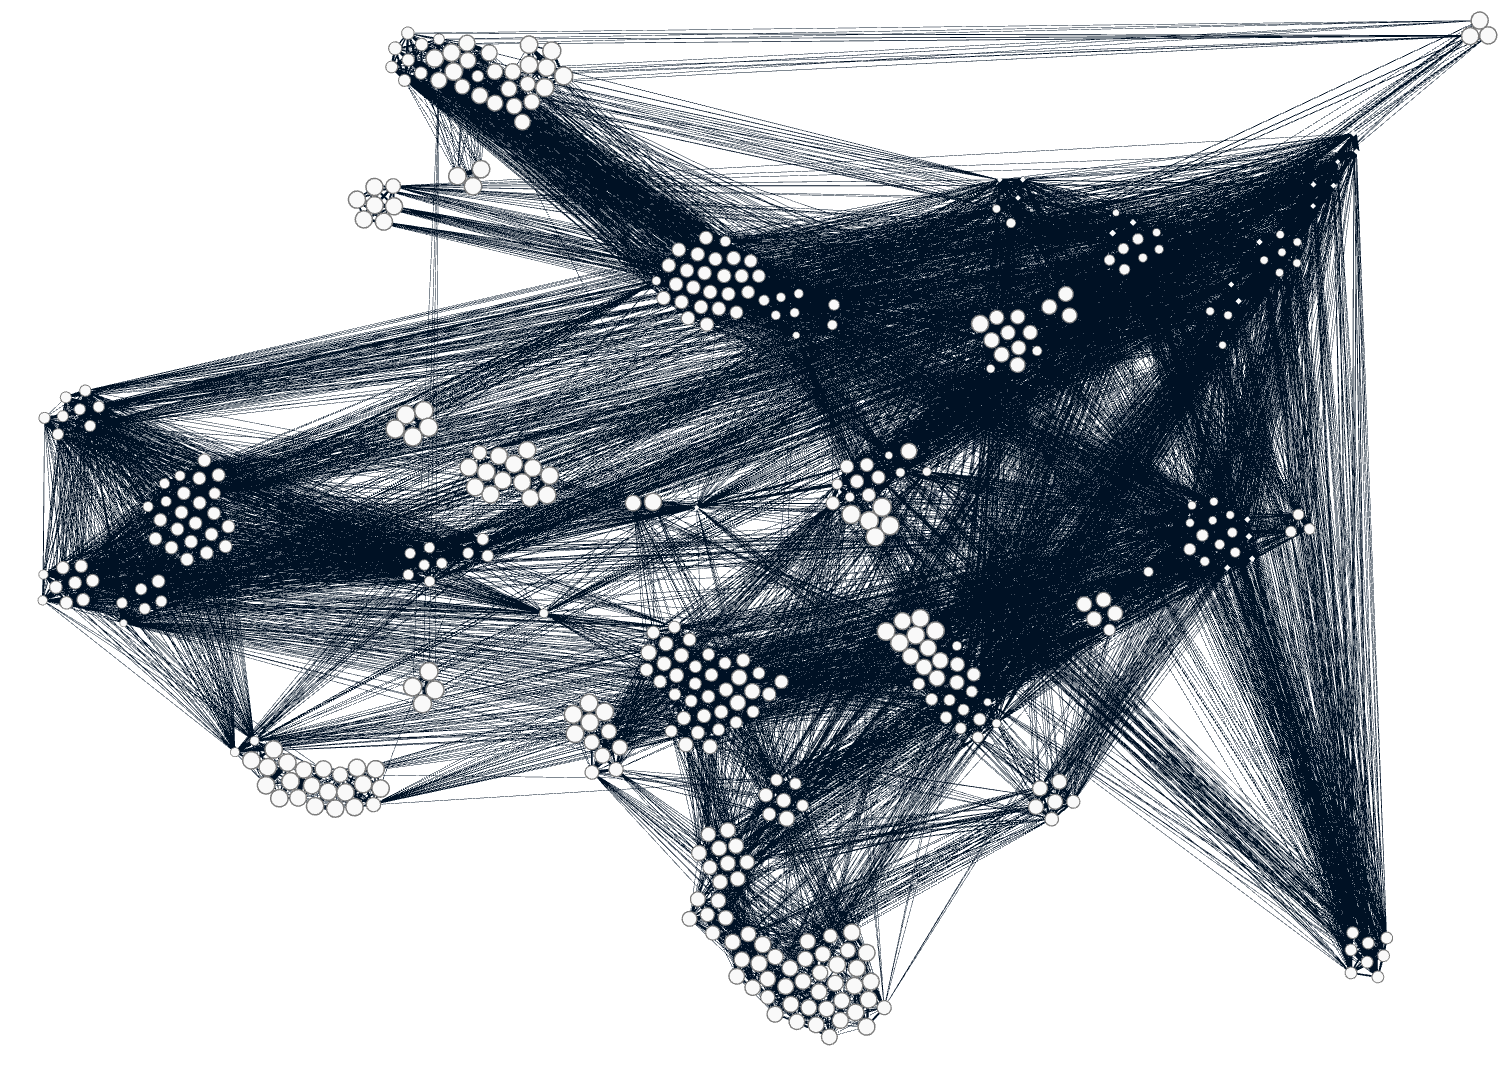
\includegraphics[width=\textwidth]{fig/c1.png}
  \caption{Full Graph}
\end{subfigure}%
\begin{subfigure}[t]{.5\textwidth}
  \centering
  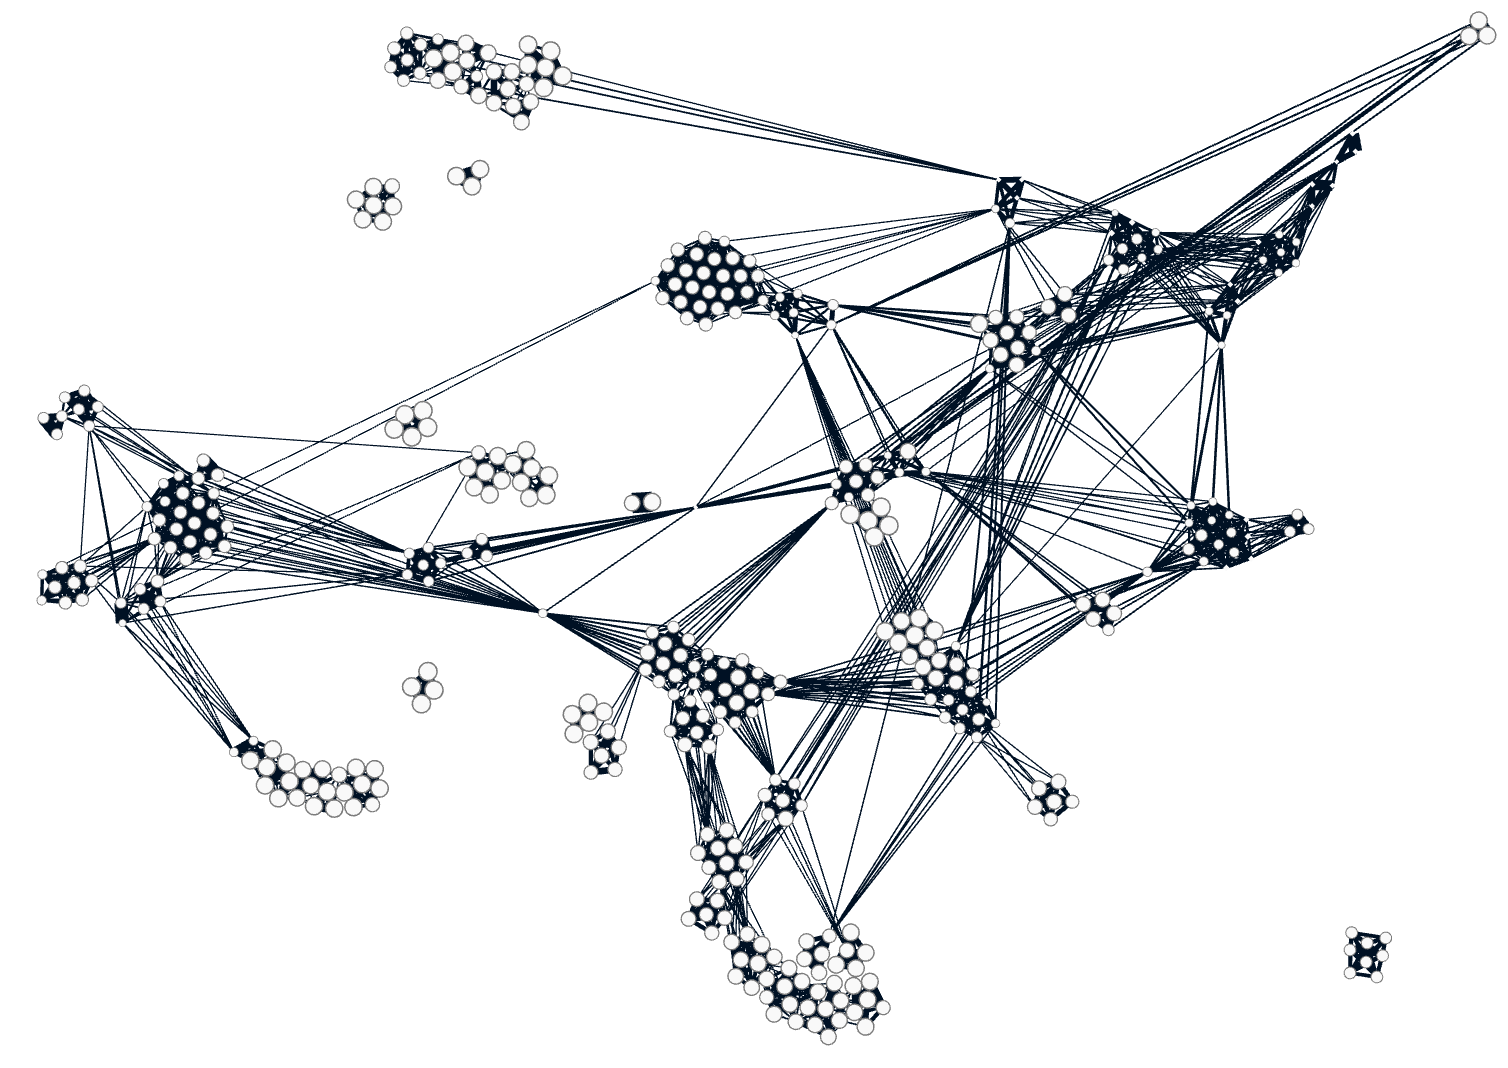
\includegraphics[width=\textwidth]{fig/c2.png}
  \caption{>10\% of graphs}
\end{subfigure}%\\

\begin{subfigure}[t]{.5\textwidth}
  \centering
  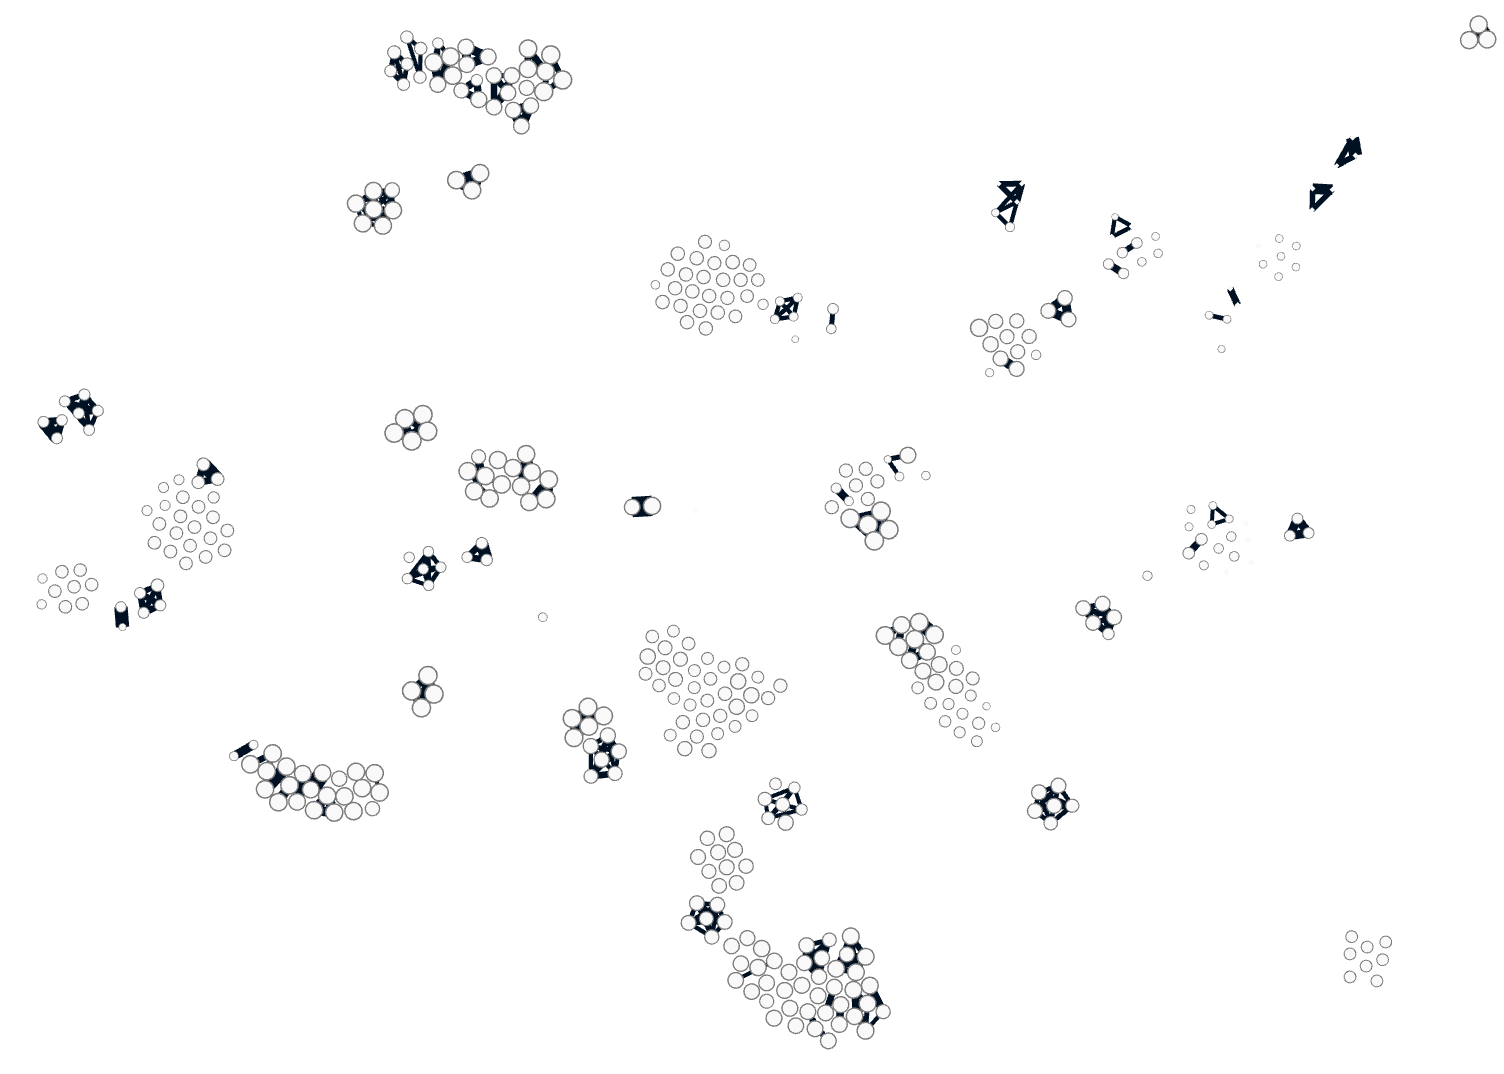
\includegraphics[width=\textwidth]{fig/c3.png}
  \caption{>20\%of graphs}
\end{subfigure}%
\begin{subfigure}[t]{.5\textwidth}
  \centering
  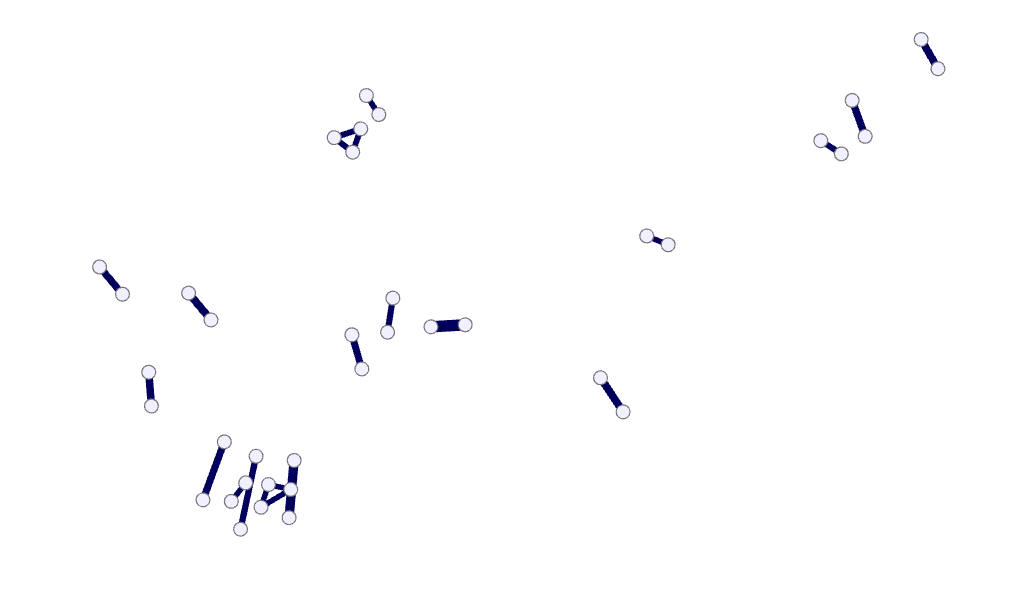
\includegraphics[width=\textwidth]{fig/c4.png}
  \caption{>40\%of graphs}
\end{subfigure}%
\caption{\textbf{Filetering the infomap clustering relationship matrix/graph} How the clutering relationship network changes as weak links (links between species which do not appear in many of the infomap groupings) are removed. }
\label{fig:infomapprune}
\end{figure}

\subsection{Comparing daytime and nightime groups}
In determing a group of species which are commonly custered together in most simulation results, we are next interested in seeing if these groups change with day or night. 

To do this we use an alluvial diagram. This is a cross between a parallel-line plot and a sanky diagram, and is particularly suitable for showing the changes in clusters within a temporal network, \citep{alluvial}.

In taking a the common clusters formed at midnight (\autoref{fig:alluvial} left)  and midday (\autoref{fig:alluvial} right) we are able to compare these to the overall selection (all hours - middle). Here, as is expected, any parings which persist in over 45\% of all the timesteps, exist in all three categories. In addition we see a selection of species which are grouped together at both 12:00 and 0:00 hours. This suggests that they may not be grouped with some of the intermediate hours, and that if the threshold of selection is lowered below 45, they may appear in the overall result. Finally a selection of species which are only grouped togehter in daytime or night time only results.



\begin{figure}%[H]
    \centering
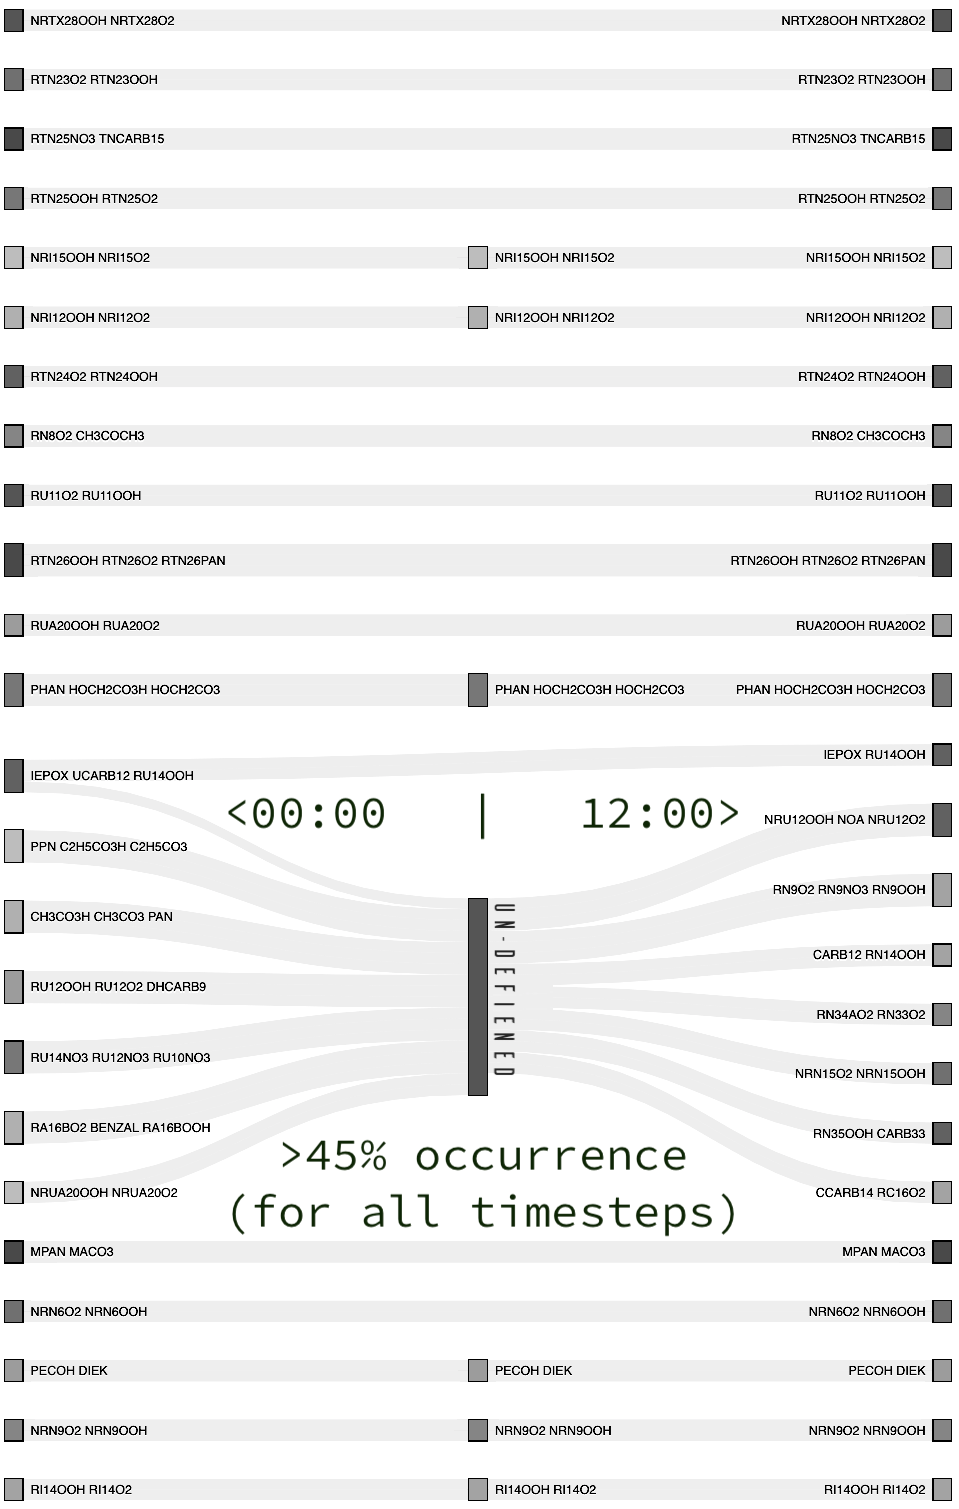
\includegraphics[width=.9\textwidth]{fig/alluvial.png}
\caption{\textbf{An alluvial diagram showing the changes in clusters between noon and midnight.} On the left are all groups that apear in >45\% of the midnight simulation results. On the right are groups which appear >45\% of the midday results. In the middle exist the clusters extracted which appear in >45\% of all runs. Here it is seen that there exist a series of species which may exist in daytime or nighttime chemistry, but do not persist between both. }
\label{fig:alluvial}
\end{figure}



\subsection{Determining cluster suitabiltiy}
Having selected clusters that appear for most graphs in the network, it is now important to assess the suitability of each node for being lumped together. Using a normalised similarity matrix, we extract the values for each of the lumbed groups, \autoref{tab:lumppair}. Here the best values are providec by the PECOH and DIEK species, \autoref{fig:lumppair}a. These both have linear decaying concentrations within the same order of magnitude. This is probably due to PECOH being the only precursor to DIEK, where DIEK accounts for 0.436\% of its total products. This makes them a suitable candidate for lumping. 
\ce{HOCH2CO3H} and \ce{HOCH2CO3} make the worst possible lumping combinations. This is because the radical \ce{HOCH2CO3} is able to react with many of the inorganics, whilst \ce{HOCH2CO3H} can only dissociate into formaldehyde or react with OH to reproduce HOCH2CO3. Although these species both have differing profiles, of several orders of magnitude difference, their cyclic nature \ce{HOCH2CO3H <=>[OH][HO2] HOCH2CO3} most likely proved to trap the `flow' of the network, producing the cluster. Additionally there are also several clusters consisting of \ce{(N)RIxxOOH} and \ce{(N)RIxxO2} species. These are genearally species formed from iso-alkanes, and both produce acetaldehyde (\ce{CH3CHO}) as a product. Here the peroxy radical (\ce{R-O2}) reacts with several inorganic species, producing a varying diurnal. Regardless of this the cosine similarity is still relatively small. This may be attributed to the `flat' periods of slow decay that is experienced at nighttime (due to the reduction of available \ce{HO2} and \ce{NO}) which follow the loss trend of the peroxide (\ce{R-OOH}) species. Since hydrogen addition and subtraction are both fast reactions forming species with the same oxidation potential (or CRI number), it makes sense that the clustering algorithm often identifies peroxides and their peroxy radical equivalent as a group. \\


\begin{table}[H]
\centering
\begin{tabular}{l|cc}
\textbf{Sepecies Pair} & \textbf{Euclidean} & \textbf{Cosine}\\
\hline\hline
NRI15OOH NRI15O2 & 0.4624 & 0.2885 \\
\hline
NRI12OOH NRI12O2 & 0.4617 & 0.2986 \\
\hline
PHAN  HOCH2CO3 & 0.5103 & 0.9998 \\
HOCH2CO3H HOCH2CO3 & 0.8350 & 0.9892 \\
\hline
RI14OOH RI14O2 & 0.4922 & 0.2275 \\
\hline
NRN9O2 NRN9OOH & 0.4620 & 0.2818 \\
\hline
PECOH DIEK & 0.0172 & 0.0011 \\
\end{tabular}
\caption{A table of the \textbf{normalised} similarity values for the lumped species. Numbers closest to 1 show the worst possible paring in the mechanism, and numbers approaching 0 show the best. }
\label{tab:lumppair}
\end{table}


\begin{figure}[H]
\begin{subfigure}[t]{.5\textwidth}
  \centering
  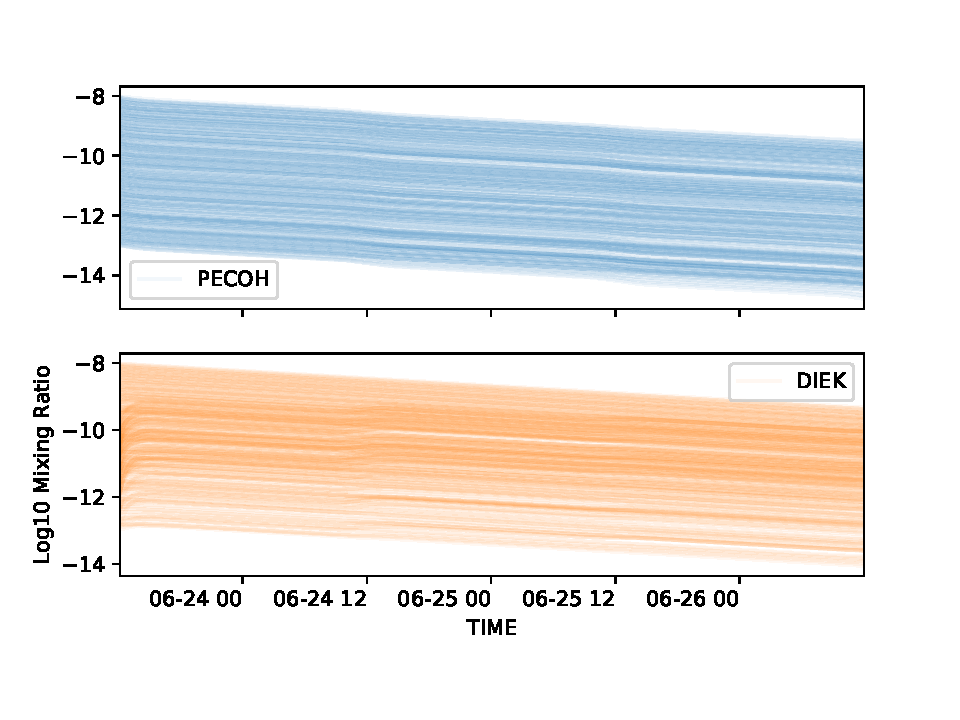
\includegraphics[width=\textwidth]{ensemble/PECOH-DIEK.pdf}
\end{subfigure}%
\begin{subfigure}[t]{.5\textwidth}
  \centering
  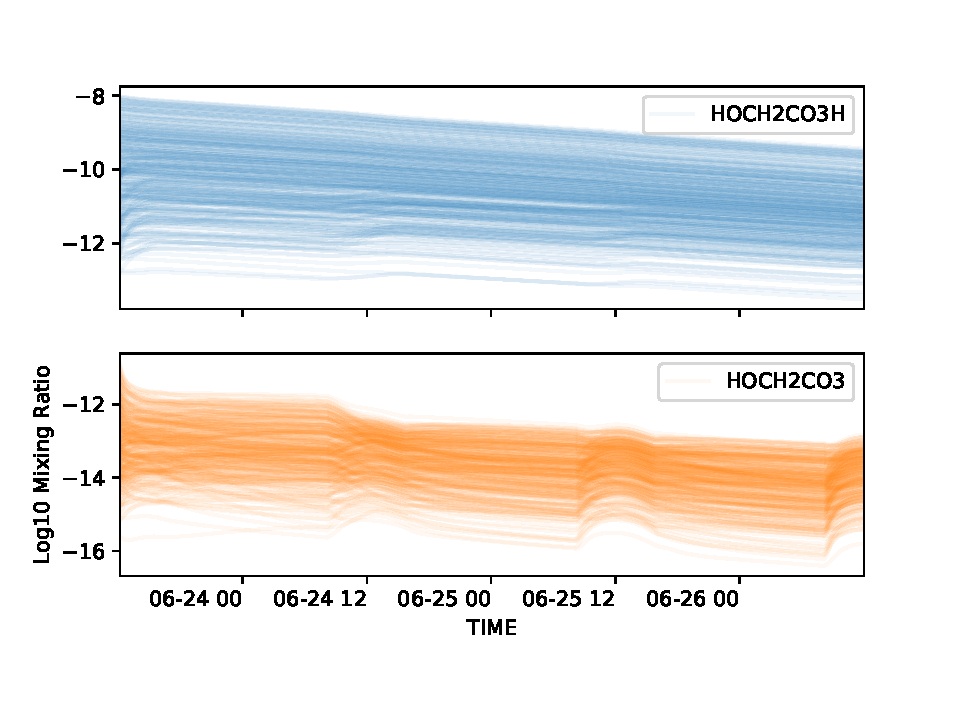
\includegraphics[width=\textwidth]{ensemble/HOCH2CO3H-HOCH2CO3.pdf}
\end{subfigure}%\\

\begin{subfigure}[t]{.5\textwidth}
  \centering
  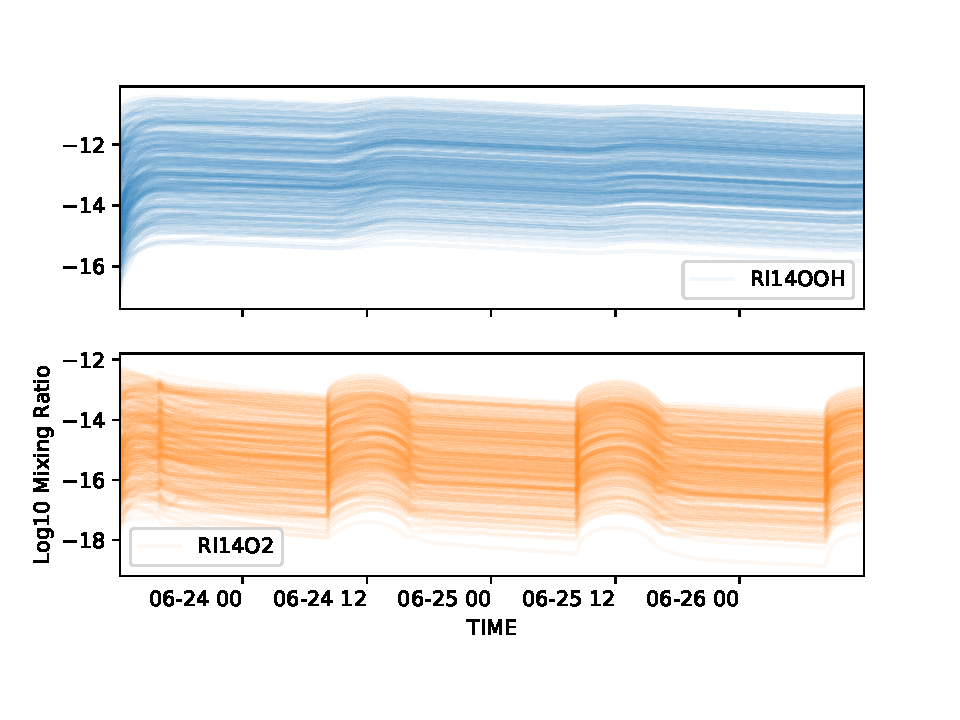
\includegraphics[width=\textwidth]{ensemble/RI14OOH-RI14O2.pdf}
\end{subfigure}%
\begin{subfigure}[t]{.5\textwidth}
  \centering
  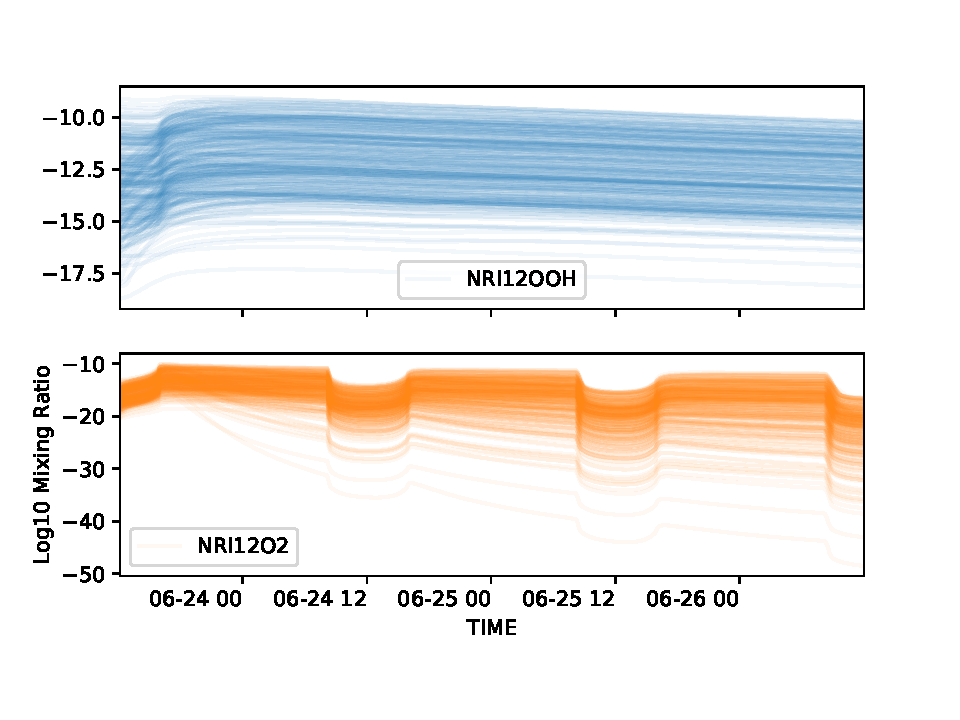
\includegraphics[width=\textwidth]{ensemble/NRI12OOH-NRI12O2.pdf}
\end{subfigure}%\\
\caption{\textbf{Comparing the best (a-b) and worst (c-d) species combinations using the combigned similarity metrics.} }
\label{fig:lumppair}
\end{figure}





% 
% 
% df.index = pd.MultiIndex.from_tuples(... 
% 
% df.euclid = df.euclid/df.euclid.max()
% df.cosine = df.cosine/df.cosine.max()
% 
% 
% 
% g = 'NRI15OOH NRI15O2,,NRI12OOH NRI12O2,,PHAN HOCH2CO3H,PHAN  HOCH2CO3,HOCH2CO3H HOCH2CO3,,RI14OOH RI14O2,,NRN9O2 NRN9OOH,,PECOH DIEK'.split(',')
% 
% 
% s =''
% for i in g:
%     try:
%         e = df.loc[tuple(sorted(i.split()))]
%         s+= '%s & %.4f & %.4f //\n'%(i,e.euclid,e.cosine)
%     except:
%         s+= ' & & //\n'
% 
% 
% print(s)
% 
% 
% g = 'NRI15OOH NRI15O2,NRI12OOH NRI12O2,PHAN HOCH2CO3H HOCH2CO3,RI14OOH RI14O2,NRN9O2 NRN9OOH,PECOH DIEK'.split(',')
% 
% 
% def get(x):
%     import zhdf
%     print (x)
%     return zhdf.new('lhs_general.h5',groupid = x,selection='spec',prodloss=False).spec.compute()
% 
% import multiprocessing as mp
% 
% gps = mp.Pool(50).map(get,range(0,300))
% 
% 
% 
% 
% g = 'RN27OOH RN37OOH,UDCARB20 UDCARB17,UDCARB14 UDCARB17,NRN9O2 NRN9OOH,PECOH DIEK'.split(',')
% 
% g = 'C2H5CO3 CH3NO3,CH3CO3 CH3NO3,MACO3 CH3NO3'.split(',')
% 
% 
% 
% g=['RTX24O2  RTX22O2']
% 
% 
% for i in g:
%     i = i.replace('-',' ').split()
%     print(i)
% 
%     plt.clf()
%     ax = 0
%     del ax
% 
%     for a in gps:
%         alpha = 0.06
%         d = np.log10(a[i])
%         try:
%             ax = d.plot(ax = ax,alpha = alpha,subplots=True,legend=False)
%         except:
%             ax=d.plot(alpha = alpha,subplots=True)
% 
%     plt.ylabel('Log10 Mixing Ratio')
%     plt.savefig('-'.join(i)+'.pdf')







\section{Conculsions}
Graph representation of a chemical network can be used to apply graph clustering techniques. Although there are a range of methods available, the infomap method proves well suited for the use on chemical mechanism. Applying this to the CRI v2.2 mechanism we were able to sucessfully partition the chemistry into branches representing the reactions between differenct chemical structures. This was seen by exploring the hierachical structure of the InfoMap output in the form of a tree. 

Additionally natural language similarity metrics can also apply to compare the temporal changes between species lifetime. Here the Euclidean distance can compare the magnitude difference between species pairs, whilst the cosine distance looks at the angle between them. Combigned these can give us indications if the lumping of two species can prove problematic. 

Finally 300 randomly initiates simulations were compared using  graph clustering. Here persistent groupings were extracted and their suitability compared using the similarity metrics and their lifetimes across the entirety of the simulation. 

Further work would involve the comparison of a mechanism lumped by this method to the unlumped version. The CRI v2.0 mechanism has a series of 5 further lumpings by * and can provide a useful comparison on how beneficial this method of mechanism reductiction fares agains more traditional methods. 
